\documentclass{article}
\usepackage{import}
\usepackage{graphicx}
\usepackage[utf8]{inputenc}
\usepackage[english]{babel}
\usepackage{amsmath}
\usepackage{biblatex}
\bibliography{ref.bib}

\title{ETERNITY: NUMBERS - Silver Ratio $(\delta_s)$}
\author{Md Hasibul Huq}
\date{July 2019}

\begin{document}               % plus the \end{document} command at the end.
\maketitle

\section{Introduction}          % This command makes a section title.

This document provides an understanding of only an irrational  number called Silver Ratio $(\delta_s)$. An irrational  number is  not  a rational  number, it is not possible to express an irrational number as a quotient of two integers.
\subsection{History}
Silver Ratio is studied from the time of Greek knowledge, which discusses the fundamental characteristics of the number system. Though it is not used by normal people intentionally. Silver ratio is the limiting of consecutive  of infinite sequence of integers, The silver ratio is presented in a Greek symbol ($\delta_s$).

\subsection{Mathematical Definition}
The value of silver ration is 2.4142135623 \cite{jdc_silver}. A ratio of the sequential sum of smaller number and twice of the larger number, which will produce an infinite sequence and the ration between smaller and larger number will be always same \cite{numberphile_silver}. This can be presented in mathematical equation:- 

\[ \dfrac{2a + b}{a}  = \dfrac{b}{a} = \delta_s \]

It will be easier to understand if it can be compared with Fibonacci number.
In Fibonacci, the smaller and larger number are added to get the next one. 
Example:-

$$1,1,2,3,5,8,13,..$$

For silver ratio, the smaller and twice of the larger number are added to get the next one. Example:-

\[1,2,5,12,29,70,..\] 

Then the latest number is divided  by the previous larger number. 

\section{Interview}

I interviewed a undergraduate student from Dhaka University - Bangladesh with math background.Her name is Esrat Jahan Tonni. As she is currently studying, she might need to use irrational numbers in her undergraduate career. The interview questions and the answers are given below:-\newline

\subsection{Question and Answer}
Q1: How long you are in math domain? \newline
Ans: Almost 3 years.\newline\newline
Q2: How often you use calculator?\newline
Ans: Very often. I mean almost daily.\newline \newline
Q3:What type of device you use to calculate complex equation.\newline
Ans:It is obviously scientific calculator for me but for advance user there are many software available.\newline\newline
Q4: Can you tell me some of the tools name?\newline
Ans: No. I can't remember the names but if you search it in Google you will find some.\newline\newline
Q5: Do you know about the irrational number?\newline
Ans: Yes. I Know,\newline\newline
Q6: Do you know about Silver Ratio?\newline
Ans: I am not sure. I think, I know about it but never used it . But have some basic idea about it. \newline\newline
Q7: Can you explain me what you know about it?\newline
Ans: I am not sure. But so far I can remember i will try to give you a basic idea of it. Hopefully you heard the name of Fibonacci number. It is related to Golden Ratio. Same as there is Silver ratio. It has some difference with golden ratio.It actually describe the twice  of the larger number added with the previous number and ratio with previous number.\newline\newline
Q8: Do you know the value of silver ratio?\newline
Ans: It is something one plus square root of two. I forget the value. It will be something 2.414 and more \newline\newline
Q9:What do you think are the applications of the Golden Ratio in mathematics?\newline
Ans: The silver ratio is used mostly in the Geometry to create designs that are in proportions. It is not used as such in Mathematics directly but even the ratio of consecutive numbers in Pell sequence are close to the silver ratio. \newline\newline
Q10: What are the other places where it can help?\newline
Ans: It is usually used in the geometrical calculation.As well as the architect and engineers uses this to make shapes calculation.It may be used in art and design, some time it helps in surgery to measure some points.  \newline\newline
Q11: Can you give me some example where it can be implemented\newline
Ans: To make a perfect square it helps. Octagon is another example where you need this.\newline\newline
Q12: Do your scientific calculator support silver ratio?\newline
Ans: Never used that. so I am not sure about it. it may be or may not be.\newline\newline
Q13: Would you like to include Irrational constants like silver ratio and others in the calculator? \newline
Ans: Yes. Why not may be in future i need them.\newline\newline
Q14: Do you have any other suggestion that can help me to find your necessity in a scientific calculator?\newline
Ans: Currently, I don't need any other feature in my calculator. but who knows if can come up with something new it may help others.\newline\newline

\subsection{Interview  Analysis}
Though the interviewee is not expert in the area of the irrational numbers, She has decent idea about the silver ratio. As she has a math background, she gave a lots of insights about the silver ratio. She is 4th Year student and completed 3 years in math domain. As a math student she has to use calculator almost everyday and she uses scientific calculator for the complex equations. From the interview, it is clear that the silver ratio is used in calculation of geometrical shapes. Also the architect, designer, engineers and Sometimes doctors (Plastic Surgery) uses this. Also stated that in regular scientific calculator the irrational numbers are not available. Then she describe about the silver ratio . which has the value of 4142135623.Its convergent are square triangular numbers, Pell numbers and octagons. According to her it will be good if the irrational numbers are included in the scientific calculator. According to him the calculation can be done here in the scientific calculators but they needs extra effort. But inclusion of these can make few peoples life easier. 

\section{Persona}
The persona is given below: 
\begin{figure}[ht!]
  
  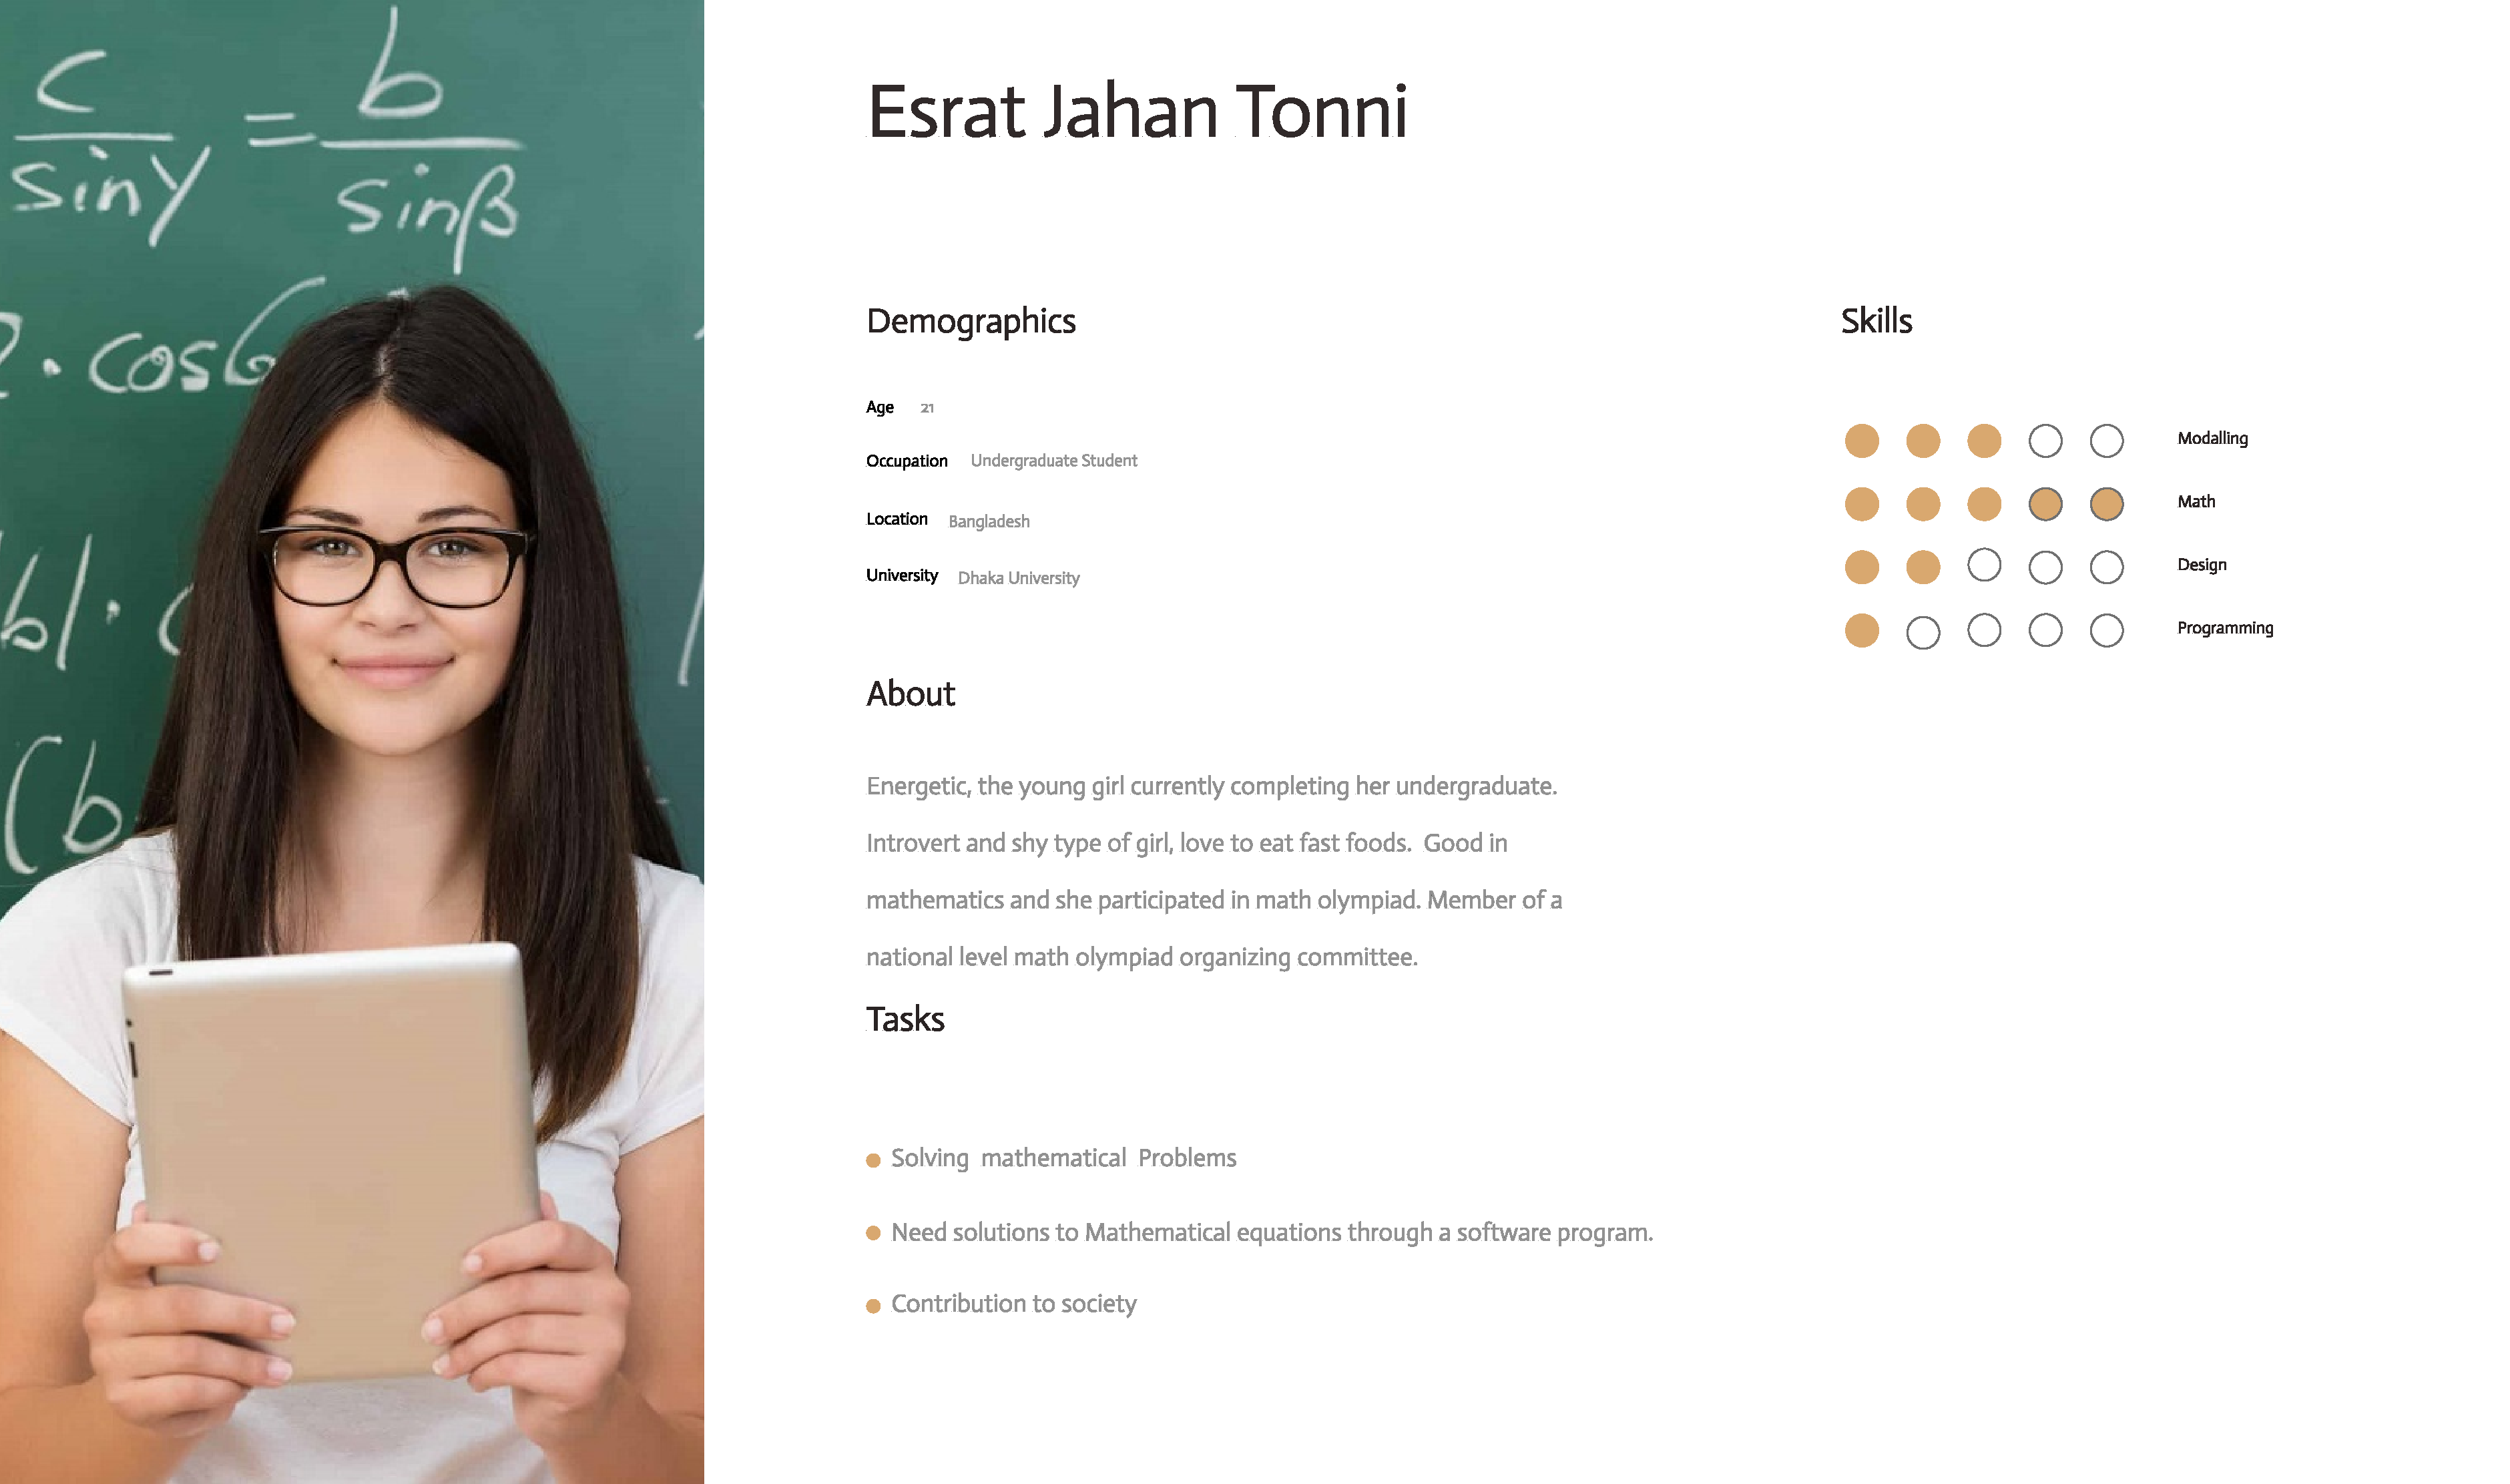
\includegraphics[width=1\textwidth]{persona}
  \centering
  \caption{Persona based on the analysis of interview}
\end{figure}

\section{Problem Domain Model}
\begin{figure}[ht!]
  
  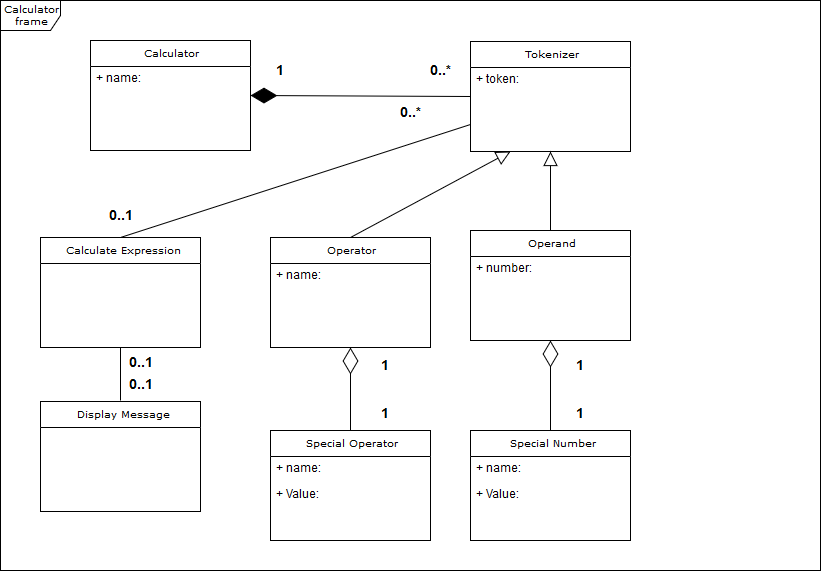
\includegraphics[width=1\textwidth]{uml}
  \centering
  \caption{Class diagram for calculator with special number and operator}
\end{figure}
\printbibliography

\end{document}                 % The input file ends with this command.
